\documentclass{article}
\usepackage[utf8]{inputenc}
\usepackage{graphicx}
\usepackage{amsfonts}       % blackboard math symbols

\setlength{\parindent}{1cm} % espaçamento do parágrafo
\usepackage{geometry} % configurar layout da página
\usepackage{setspace} % configurar o espaçamento de linhas
\usepackage{indentfirst} % alinhamento do texto, parágrafos

\graphicspath{ {./images/} }

\usepackage{float} % tabela que nao fica fixa

\usepackage{siunitx}  % Package perfeita pra notacao cientifica
\RequirePackage{amsmath,amsthm,amssymb,hyperref} % Math 

\title{ENGC46 - Síntese de Circuitos: Trabalho II}
\date{Semestre Letivo Suplementar 2020 - Universidade Federal da Bahia}
\author{Henrique Nunes Poleselo}

\begin{document}

\maketitle

\section{Especificações}
O objetivo é projetar um filtro passa-baixas utilizando redes passivas e depois converte-lo em rede ativa utilizando a transformação de Bruton de forma a eliminar os indutores da rede passiva. As seguintes especificações:
\begin{itemize} 
    \item Banda passante: 0Hz - 28kHz
    \item Banda de rejeição: 28kHz - 123.3kHz
    \item Amax: 0.1dB
    \item Amin: 40dB
    \item Impedância de carga e da fonte: 1k
    \item Função de aproximação: Butterworth
    \item Técnica de Bruton
\end{itemize}


\section{Projeto}

A ordem mínima para a realização do filtro foi de n = 5. Foi utilizado

\begin{equation}
    T(s) = Kmax \cdot \frac{ s^2 + wo^2 }{s^2 + \frac{wo}{Q} s + wo^2}.
\end{equation}

\begin{equation}
    \frac{RPA}{RPB \cdot R^2 \cdot C^2} = \num{1.105e11}
\end{equation}

\begin{table}[H]
\centering
\begin{tabular}{|c|c|c|}
\hline
Componente & Normalizado  & Desnormalizado  \\ \hline
C1 & \num{0.4243}F & \num{2.41e-9}F \\ \hline
C3 & \num{1.3732}F & \num{7.805e-9}F \\ \hline
C5 & \num{0.4243}F & \num{2.41e-9}F \\ \hline
L2 & \num{1.1109}H & \num{6.314e-3}H \\ \hline
L4 & \num{1.1109}H & \num{6.314e-3}H \\ \hline
\end{tabular}
\caption{Valores normalizados e desnormalizados de acordo com a frequência de corte \textit{fp} de 28kHz e impedância de 1k\si{\ohm}.}
\end{table}

A rede passica LC montada no LTSpice com os valores desnormalizados foi:
\begin{center}
\centering
  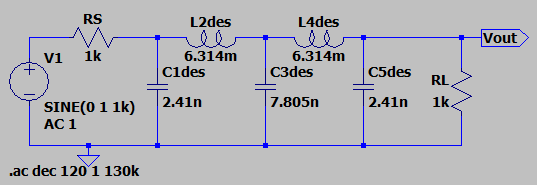
\includegraphics[scale=0.8]{img/ladder.png}
\end{center}

Como uma das especificações era de 0.1dB na banda passante, os valores extraídos. Os valores extraídos da simulação:


O circuito montado no LTSpice foi:
\begin{center}
\centering
  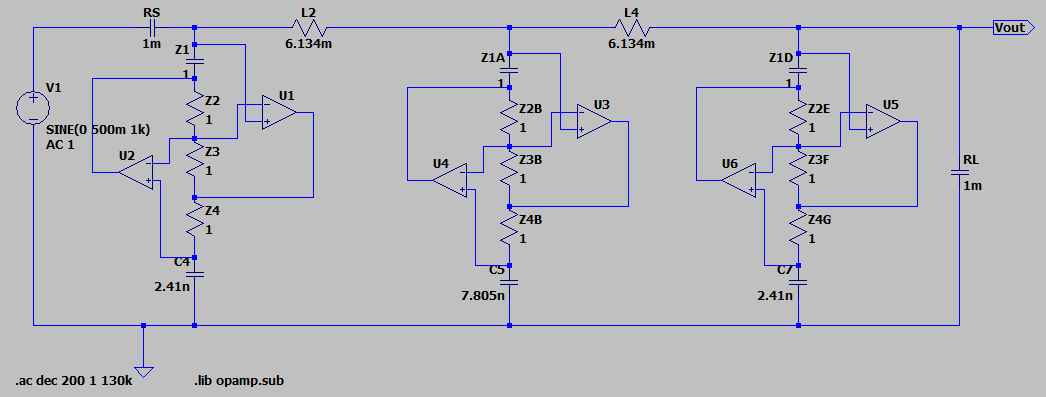
\includegraphics[scale=0.5]{img/passivoativo.png}
\end{center}


Comparação entre a rede passiva LC e a rede ativa transformada:
\begin{center}
\centering
  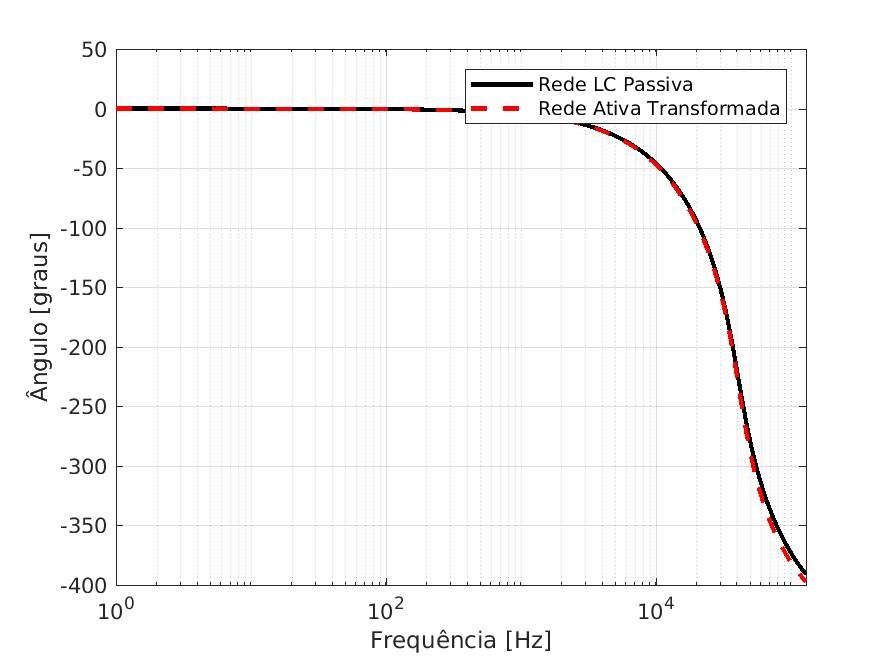
\includegraphics[scale=0.5]{img/phase.png}
\end{center}

\begin{center}
\centering
  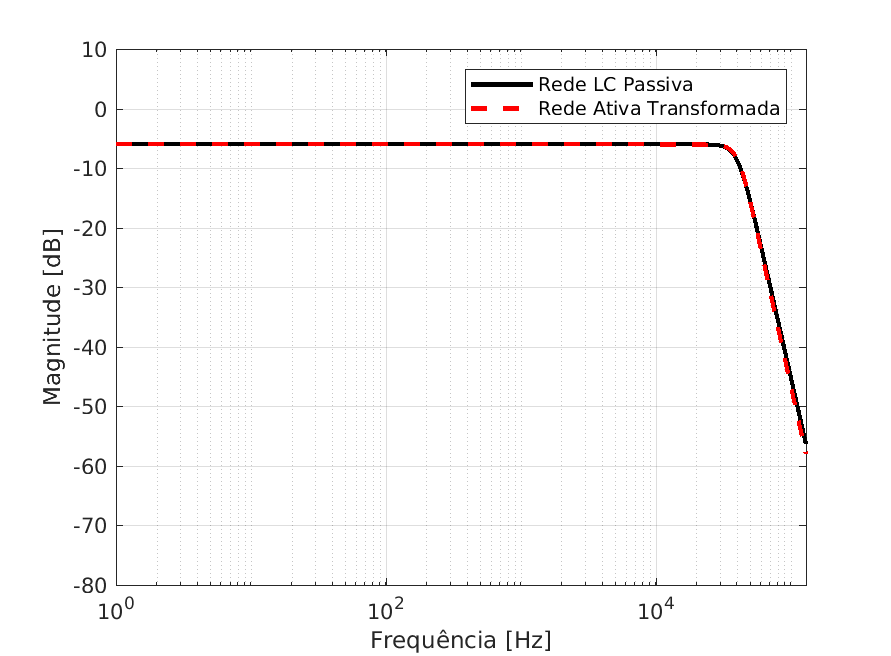
\includegraphics[scale=0.5]{img/magnitude.png}
\end{center}



\end{document}